\section{Teorema de Thévenin. Teorema de Norton}

\frame{
	\frametitle{Teorema de Thévenin}
	\begin{block}{Introdução}
		Muitas vezes pode acontecer de um determinado elemento em um circuito ser \textbf{variável} (normalmente, denominado \textbf{carga}), enquanto outros elementos são fixos. Um exemplo característico é uma tomada de uma casa onde é possível conectar diversos aparelhos diferentes, constituindo uma carga variável.
	\end{block}
}

\frame{
	\frametitle{Teorema de Thévenin}
	\begin{block}{Importância}
		Toda vez que a carga for alterada, todo o circuito tem de ser \textbf{analisado novamente}. Para evitar esse problema, o \textbf{teorema de Thévenin} fornece uma técnica pela qual a \textbf{parte fixa} do circuito é substituída por um \textbf{circuito equivalente}.
		\vspace{-0.1cm}
		\centerline{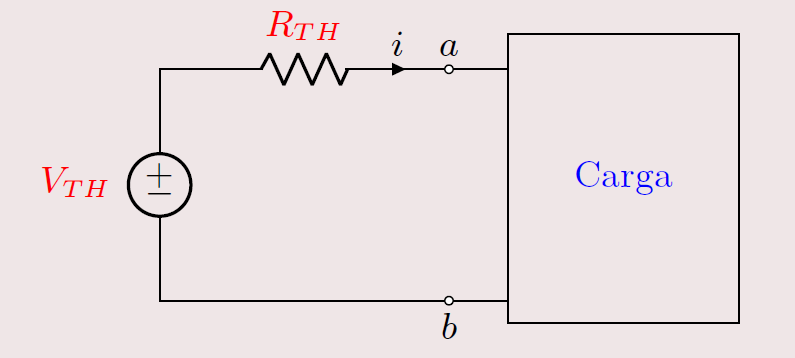
\includegraphics[width=0.6\linewidth]{Figuras/Ch05/fig1.PNG}}
		\vspace{-0.1cm}
		\begin{itemize}
			\item A \textcolor{blue}{carga} pode ser um simples resistor ou um trecho de um circuito.
			\item À esquerda de $a-b$ é conhecido como \textcolor{red}{circuito equivalente de Thévenin}.
		\end{itemize}
	\end{block}
}



\frame{
	\frametitle{Teorema de Thévenin}
	\begin{block}{O teorema}
		O \textbf{teorema de Thévenin} afirma que um circuito linear de dois terminais pode ser substituído por um circuito equivalente formado por uma \textbf{fonte de tensão} $V_{TH}$ em série com um \textbf{resistor} $R_{TH}$, onde $V_{TH}$ é a tensão de circuito aberto nos terminais; e $R_{TH}$ é a resistência de entrada ou equivalente nos terminais quando as fontes de independentes forem desativadas.
	\end{block}
}

\frame{
	\frametitle{Teorema de Thévenin}
	\begin{block}{Etapas}
		\textbf{No Teorema de Thévenin estamos interessados em encontrar $V_{TH}$ e $R_{TH}$}. Dado um circuito, faça:
		
		\begin{enumerate}
			\item Para encontrar a \textbf{tensão} $V_{TH}$ deve-se \textbf{abrir o circuito} nos terminais $a-b$, eliminando-se a carga. $V_{TH}$ é a tensão de circuito aberto nos terminais.
			\saveenumerate
		\end{enumerate}
	
		$$V_{TH} = V_{ab}$$
	\end{block}
}

\frame{
	\frametitle{Teorema de Thévenin}
	\begin{block}{Etapas}
		\textbf{No Teorema de Thévenin estamos interessados em encontrar $V_{TH}$ e $R_{TH}$}. Dado um circuito, faça:
		
		\begin{enumerate}
			\restoreenumerate
			\item Para encontrar a \textbf{resistência} $R_{TH}$ deve-se \textbf{desconectar os terminais em circuito aberto e desligar todas as fontes}. Portanto, $R_{TH}$ é a resistência de entrada nos terminais quando as fontes independentes forem desligadas.
		\end{enumerate}
	
		$$R_{TH} = R_{\text{ent}}$$
	\end{block}
}

\frame{
	\frametitle{Teorema de Thévenin - Exemplo \#01}
	\centerline{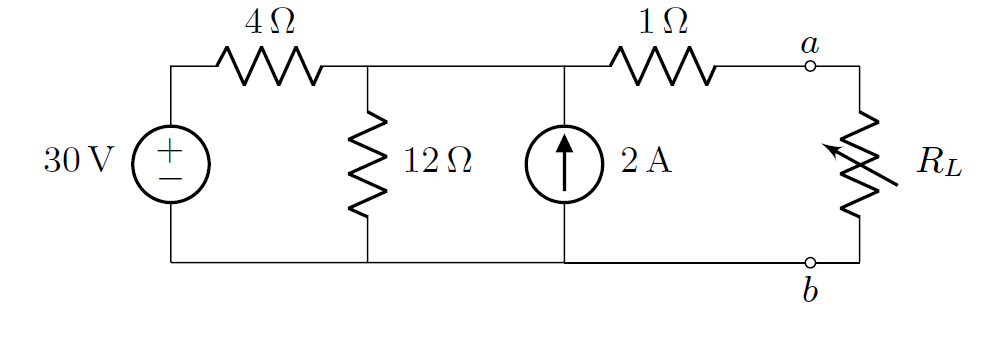
\includegraphics[width=0.9\linewidth]{Figuras/Ch05/fig2.PNG}}
}

\frame{
	\frametitle{Teorema de Thévenin - Exemplo \#01}
	\begin{block}{Resolução - \textbf{Determinar $V_{TH}$}}
		\centerline{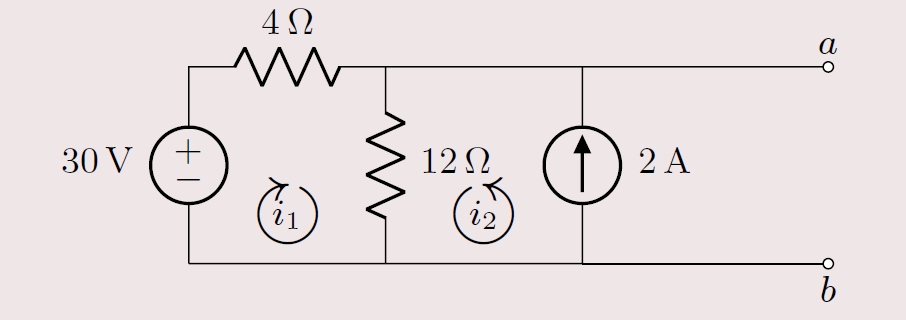
\includegraphics[width=0.7\linewidth]{Figuras/Ch05/fig3.PNG}}
		\vspace{-0.2cm}

		\textbf{Malha 1}:
		\vspace{-0.2cm}
		$$32 - 4 \cdot i_1 - 12 \cdot (i_1 + i_2) = 0$$
		$$4 \cdot i_1 + 3 \cdot i_2 = 8$$

		\textbf{Malha 2}:
		\vspace{-0.2cm}
		$$i_2 = \SI{2}{\ampere}$$ \\

		\vspace{0.2cm}

		Logo, $4 \cdot i_1 + 3 \cdot 2 = 9 \implies i_1 = \SI{0.5}{\ampere} $ \\
		\vspace{0.1cm}
		Com isso, $V_{TH} = V_{\SI{12}{\ohm}} = 12 \cdot (i_1 + 1_2) = 12 \cdot \num{2,5} = \boxed{\SI{30}{\volt}}$

	\end{block}
}

\frame{
	\frametitle{Teorema de Thévenin - Exemplo \#01}
	\begin{block}{Resolução - \textbf{Determinar $R_{TH}$}}
		\centerline{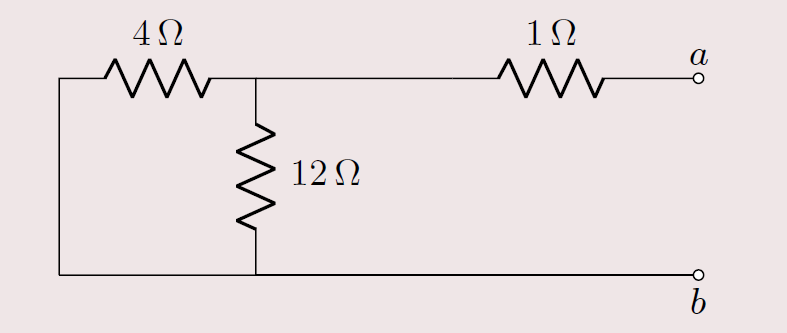
\includegraphics[width=0.7\linewidth]{Figuras/Ch05/fig4.PNG}}
		\vspace{-0.2cm}

		$$R_{TH} = (4 \parallel 12) + 1 = 3 + 1 = \boxed{\SI{4}{\ohm}}$$
	\end{block}
}

\frame{
	\frametitle{Teorema de Thévenin - Exemplo \#01}
	\begin{block}{Resolução}
		\centerline{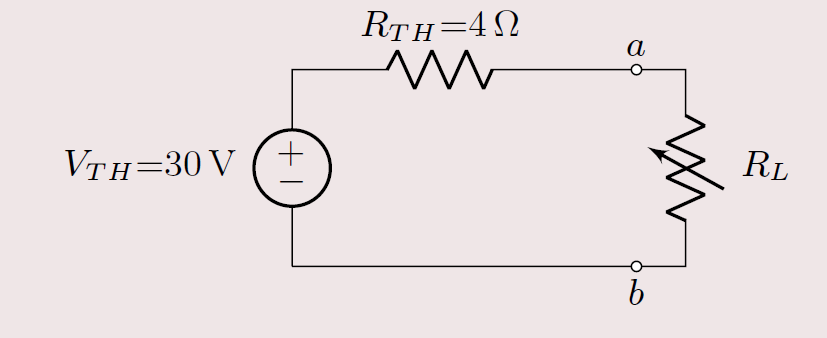
\includegraphics[width=0.7\linewidth]{Figuras/Ch05/fig5.PNG}}

		Considerando $R_L = \SI{6}{\ohm}$, temos que a corrente na carga é:

		$$i_L = \dfrac{30}{4+6} = \SI{10}{\ampere}$$
	\end{block}
}


\frame{
	\frametitle{Teorema de Norton}
	\begin{block}{Introdução}
		Após cerca de 43 anos da publicação do Teorema de Thévenin, \textbf{Norton}, engenheiro norte-americano, propôs um teorema semelhante.
	\end{block}
}

\frame{
	\frametitle{Teorema de Norton}
	\begin{block}{Importância}
		Toda vez que a carga for alterada, todo o circuito tem de ser \textbf{analisado novamente}. Para evitar esse problema, o \textbf{teorema de Norton} fornece uma técnica pela qual a \textbf{parte fixa} do circuito é substituída por um \textbf{circuito equivalente}.
		\centerline{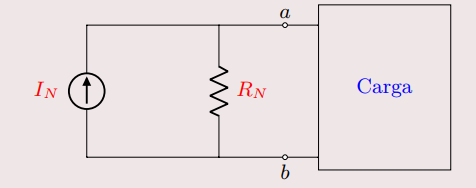
\includegraphics[width=0.7\linewidth]{Figuras/Ch05/fig6.PNG}}
		\begin{itemize}
			\item A \textcolor{blue}{carga} pode ser um simples resistor ou um trecho de um circuito.
			\item À esquerda de $a-b$ é conhecido como \textcolor{red}{circuito equivalente de Norton}.
		\end{itemize}
	\end{block}
}



\frame{
	\frametitle{Teorema de Norton}
	\begin{block}{O teorema}
		O \textbf{teorema de Norton} afirma que um circuito linear de dois terminais pode ser substituído por um circuito equivalente formado por uma \textbf{fonte de corrente} $I_{N}$ em paralelo com um \textbf{resistor} $R_{N}$, onde $I_{N}$ é a corrente de curto-circuito através dos terminais; e $R_{N}$ é a resistência de entrada ou equivalente nos terminais quando as fontes de independentes forem desativadas.
	\end{block}
}

\frame{
	\frametitle{Teorema de Norton}
	\begin{block}{Etapas}
		\textbf{No Teorema de Norton estamos interessados em encontrar $I_{N}$ e $R_{N}$}. Dado um circuito, faça: \\
		\begin{enumerate}
			\item Para descobrir a \textbf{corrente} $I_{N}$, determinamos a \textbf{corrente de curto circuito} que flui entre os terminais $a-b$.
			      \saveenumerate
		\end{enumerate}
		$$I_{N} = I_{sc}$$
	\end{block}
}

\frame{
	\frametitle{Teorema de Norton}
	\begin{block}{Etapas}
		\textbf{No Teorema de Norton estamos interessados em encontrar $I_{N}$ e $R_{N}$}. Dado um circuito, faça: \\
		\begin{enumerate}
			\restoreenumerate
			\item Para encontrar a \textbf{resistência} $R_{N}$ fazemos da mesma maneira que fazemos para $R_{TH}$. As resistências de Thévenin e Norton são \textbf{iguais}.
		\end{enumerate}
		$$R_{N} = R_{TH}$$
	\end{block}
}

\frame{
	\frametitle{Teorema de Norton x Teorema de Thévenin}
	\begin{block}{Relação}
		Existe uma estreita \textbf{relação} entre os dois teoremas:
		$$\boxed{R_{TH} = R_N}$$
		$$\boxed{I_N = \dfrac{V_{TH}}{R_{TH}}}$$
	\end{block}
}

\frame{
	\frametitle{Teorema de Norton - Exemplo \#01}
	\centerline{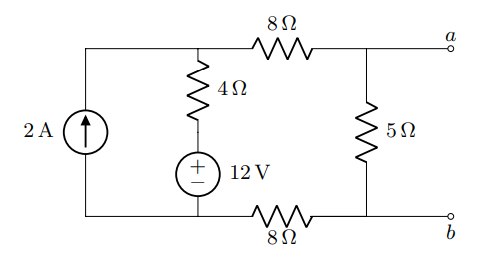
\includegraphics[width=0.7\linewidth]{Figuras/Ch05/fig7.PNG}}
}

\frame{
	\frametitle{Teorema de Norton - Exemplo \#01}
	\begin{block}{Resolução - \textbf{Determinar $I_{N}$}}
		\centerline{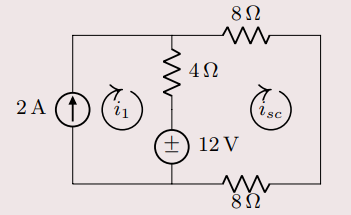
\includegraphics[width=0.5\linewidth]{Figuras/Ch05/fig8.PNG}}

		\textbf{Malha 1}:
		\vspace{-0.2cm}
		$$i_1 = \SI{2}{\ampere}$$

		\textbf{Malha 2}:
		\vspace{-0.2cm}
		$$12 - 4 \cdot (i_{sc} - i_1) - 16 \cdot i_{sc} = 0$$
		$$i_1 - 5 \cdot i_{sc} = -3$$\\

		\vspace{0.2cm}

		Logo, $2 - 5 \cdot i_{sc} = - 3 \implies i_{sc} = I_N = \boxed{\SI{1}{\ampere}}$ \\
	\end{block}
}

\frame{
	\frametitle{Teorema de Norton - Exemplo \#01}
	\begin{block}{Resolução - \textbf{Determinar $R_{N}$}}
		\centerline{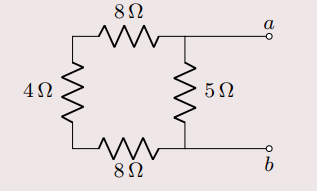
\includegraphics[width=0.5\linewidth]{Figuras/Ch05/fig9.PNG}}

		$$R_{N} = (8 + 4 + 8) \parallel 5 = 20 \parallel 5 = \boxed{\SI{4}{\ohm}}$$
	\end{block}
}

\frame{
	\frametitle{Teorema de Norton - Exemplo \#01}
	\begin{block}{Resolução}
		\centerline{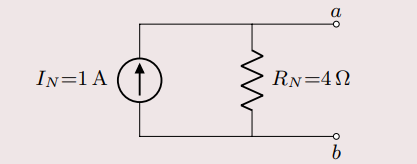
\includegraphics[width=0.6\linewidth]{Figuras/Ch05/fig10.PNG}}
	\end{block}
}

\section*{Exercícios}
\frame{
	\frametitle{Exercícios}
	\begin{block}{}
		01. Usando o teorema de Thévenin, determine o circuito equivalente à esquerda dos terminais do circuito abaixo. Em seguida ache $i$.
		\centerline{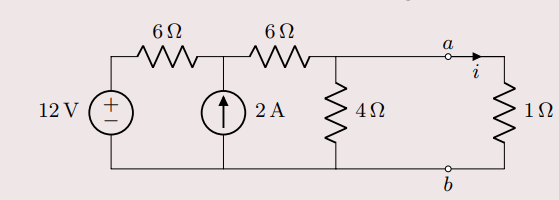
\includegraphics[width=0.9\linewidth]{Figuras/Ch05/fig11.PNG}}
	\end{block}
}

\section*{Exercícios}
\frame{
	\frametitle{Exercícios}
	\begin{block}{}
		02. Determine o equivalente de Norton para o circuito abaixo nos terminais $a-b$.
		\centerline{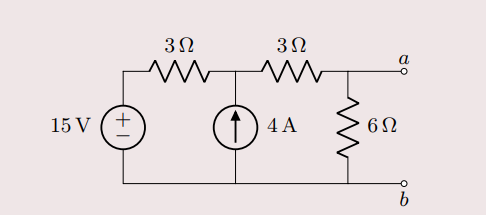
\includegraphics[width=0.8\linewidth]{Figuras/Ch05/fig12.PNG}}
	\end{block}
}

\section*{Referências}

\frame{
	\frametitle{Referências e Exercícios Complementares}
	\begin{itemize}
		\item ALEXANDRE, Charles K.; SADIKU, Matthew N. O. Fundamentos de Circuitos Elétricos. 5. ed. Porto Alegre: AMGH, 2013.
	\end{itemize}
	%\centering{\alert{Página 36 - \textbf{1.6.1 até 1.6.5, 1.6.17 até 1.6.19}}} \\
	\centering{\alert{Lista de exercícios 05}}
}